\normaltrue \difficilefalse \tdifficilefalse
\correctiontrue

%\UPSTIidClasse{11} % 11 sup, 12 spé
%\newcommand{\UPSTIidClasse}{12}

\exer{Système bielle manivelle  $\star\star$ \label{C2:06:12}}
\setcounter{question}{0}\UPSTIcompetence[2]{C2-06}
\index{Compétence C2-06}
\index{Bielle Manivelle}
\index{Moteur}
\ifcorrection
\else
\marginnote{\textbf{Pas de corrigé pour cet exercice.}}
\fi

\ifprof
\else
Soit le mécanisme suivant. On a $\vect{AB}=R\vect{i_1}$, $\vect{CB}=L\vect{i_2}$ et $\vect{AC}=\lambda(t) \vect{j_0}$. 

\begin{center}
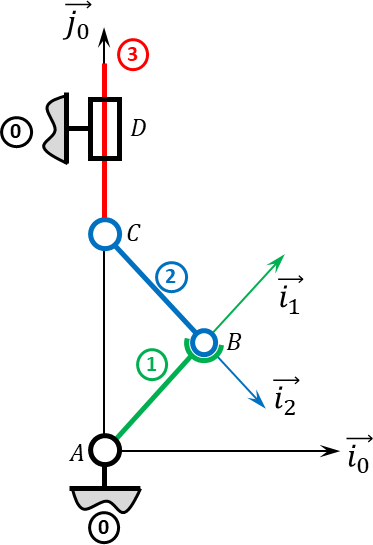
\includegraphics[width=\linewidth]{12_01}
\end{center}
\fi

\question{Tracer le graphe des liaisons.}

\ifprof
\begin{center}
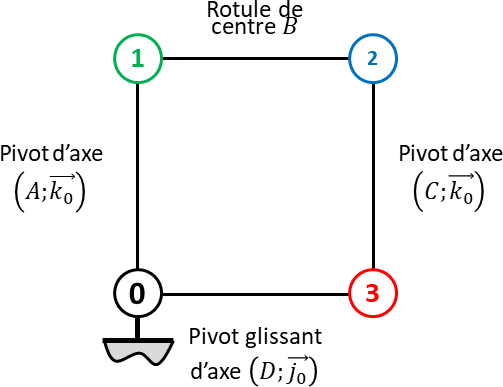
\includegraphics[width=.4\linewidth]{12_01_c}
\end{center}
\else
\fi

\question{Exprimer $\lambda(t)$ en fonction de $\theta(t)$.}

\ifprof
En réalisant une fermeture géométrique, on obtient 
$\vect{AB}+\vect{BC}+\vect{CA}=\vect{0}$ 
$ \Leftrightarrow R\vect{i_1} - L\vect{i_2} - \lambda(t) \vect{j_0} = \vect{0}$.
On projette alors cette expression dans $\rep{0}$ : 

$
\left\{
\begin{array}{l}
R\cos\theta(t)- L\cos\varphi(t) = 0 \\
R\sin\theta(t) - L\sin\varphi(t) - \lambda(t) = 0 
\end{array}
\right.
$.

On cherche à éliminer $\varphi(t)$ : 

$
\left\{
\begin{array}{l}
R\cos\theta(t) = L\cos\varphi(t)  \\
R\sin\theta(t)  - \lambda(t) = L\sin\varphi(t)
\end{array}
\right.
$.

En élevant au carré, on a donc 

$\left\{
\begin{array}{l}
R^2\cos^2\theta(t) = L^2\cos^2\varphi(t)  \\
\left(R\sin\theta(t)  - \lambda(t)\right)^2 = L^2\sin^2\varphi(t)
\end{array}
\right.
$.

En conséquence, 
$R^2\cos^2\theta(t)  + \left(R\sin\theta(t)  - \lambda(t)\right)^2 = L^2$ et 

$ \left(R\sin\theta(t)  - \lambda(t)\right)^2 = L^2 - R^2\cos^2\theta(t) $ 
$\Rightarrow    \lambda(t) = \pm\sqrt{L^2 - R^2\cos^2\theta(t)} + R\sin\theta(t) $ .
\else
\fi

\question{Exprimer $\dot{\lambda}(t)$ en fonction de $\dot{\theta}(t)$.}
\ifprof

$\lambdap(t) = \pm\left( \dfrac{R^2 \thetap(t) \cos\theta(t)\sin\theta(t)}{\sqrt{L^2 - R^2\cos^2\theta(t)}}\right) + \thetap(t)R\cos\theta(t) $ 

\else
\fi

\question{En utilisant Python, tracer la vitesse du piston en fonction du temps. La fréquence de rotation est $\dot{\theta}(t)=\SI{100}{rad.s^{-1}}$, on prendra $R=\SI{10}{mm}$ et $L=\SI{20}{mm}$ puis $L=\SI{30}{mm}$.}

\ifprof
\noindent\hrule
\begin{lstlisting}
#!/usr/bin/env python
# -*- coding: utf-8 -*-

"""12_BielleManivelle.py"""
__author__ = "Xavier Pessoles"
__email__ = "xpessoles.ptsi@free.fr"

import numpy as np
import matplotlib.pyplot as plt
import math as m
from scipy.optimize import newton
from scipy.optimize import fsolve

R = 0.01 # m
L = 0.03 # m
w = 100
def calc_lambda(theta):
    #res = R*np.sin(theta)
    #print(L*L-R*R*np.cos(theta)*np.cos(theta))
    #res = res + np.sqrt(L*L-R*R*np.cos(theta)*np.cos(theta))
    res = np.sqrt(L*L-R*R*np.cos(theta)*np.cos(theta))+R*np.sin(theta)
    return res

def plot_lambda():
    les_theta=np.linspace(-2*np.pi,2*np.pi,1000)
    les_l = [calc_lambda(x) for x in les_theta]
    plt.grid()
    plt.xlabel("Temps (s)")
    plt.ylabel("Vitesse (${m}s^{-1}$)")
    plt.plot(les_theta,les_l,label=str("R=")+str(R)+" mm,"+str("L=")+str(L)+" mm")
    plt.legend()
    plt.show()
    
plot_lambda()
\end{lstlisting}
\noindent\hrule

\begin{center}
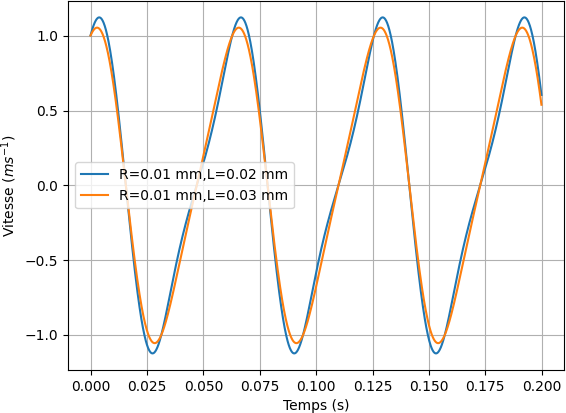
\includegraphics[width=.4\linewidth]{12_02_c}
\end{center}
\else
\fi

\question{En utilisant Python, tracer l'accélération du piston en fonction du temps en utilisant les mêmes valeurs que dans la question précédente. On utilisera une dérivation numérique.}

\ifprof
\begin{center}
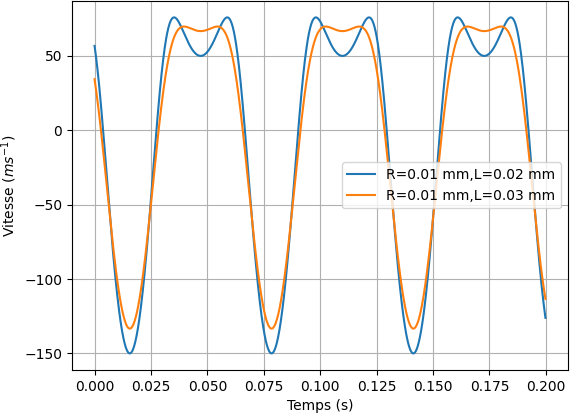
\includegraphics[width=.4\linewidth]{12_03_c}
\end{center}
\else
\fi



\ifprof
\else
\footnotesize
\ifcolle
\else
\begin{center}
\begin{tabular}{|p{.9\linewidth}|}
\hline
Indications :
\begin{enumerate}
\item .
\item $\lambda(t) = \pm\sqrt{L^2 - R^2\cos^2\theta(t)} + R\sin\theta(t) $.
\item $\lambdap(t) = \pm\left( \dfrac{R^2 \thetap(t) \cos\theta(t)\sin\theta(t)}{\sqrt{L^2 - R^2\cos^2\theta(t)}}\right) + \thetap(t)R\cos\theta(t)$.
\item .
\item .
\end{enumerate} \\ \hline
\end{tabular}
\end{center}
\fi
\normalsize
\begin{flushright}
\footnotesize{Corrigé  voir \ref{C2:06:12}.}
\end{flushright}%
\fi